\documentclass[11pt]{article}
\usepackage[margin=1in, top=1in]{geometry}
\usepackage[all]{nowidow}
\usepackage[hyperfigures=true, hidelinks, pdfhighlight=/N]{hyperref}
\usepackage[separate-uncertainty=true, group-digits=true]{siunitx}
\usepackage{graphicx,amsmath,physics,tabto,float,amssymb,pgfplots,verbatim,tcolorbox}
\usepackage{listings,xcolor,subfig,caption,import,wrapfig,enumitem}
\usepackage[version=4]{mhchem}
\usepackage[noabbrev]{cleveref}
\newcommand{\creflastconjunction}{, and\nobreakspace}
\newcommand{\mb}[1]{\mathbf{#1}}
\definecolor{stringcolor}{HTML}{C792EA}
\definecolor{codeblue}{HTML}{2162DB}
\definecolor{commentcolor}{HTML}{4A6E46}
\captionsetup{font=small, belowskip=0pt}
\lstdefinestyle{appendix}{
    basicstyle=\ttfamily\footnotesize,commentstyle=\color{commentcolor},keywordstyle=\color{codeblue},
    stringstyle=\color{stringcolor},showstringspaces=false,numbers=left,upquote=true,captionpos=t,
    abovecaptionskip=12pt,belowcaptionskip=12pt,language=Python,breaklines=true,frame=single}
\lstdefinestyle{inline}{
    basicstyle=\ttfamily\footnotesize,commentstyle=\color{commentcolor},keywordstyle=\color{codeblue},
    stringstyle=\color{stringcolor},showstringspaces=false,numbers=left,upquote=true,frame=tb,
    captionpos=b,language=Python}
\renewcommand{\lstlistingname}{Appendix}
\pgfplotsset{compat=1.17}

\begin{document}

\begin{center}
    \textbf{CP Exam}\hspace{1.5in}\textbf{KDSMIL001}\hspace{1.5in}\textbf{11-06-2022}
\end{center}
\rule{\textwidth}{1pt}

\begin{enumerate}
    \item \begin{enumerate}
        \item We generate \num[]{20000} random numbers according to the Gaussian distribution with form 
        \begin{equation}
            P_{\mathrm{Gaussian}}(N,\langle N \rangle)=\frac{1}{\sqrt{2\pi\langle N \rangle}}\exp\left(-\frac{(N-\langle N \rangle)^2}{2\langle N \rangle}\right)
            \label{eqn:gaussian}
        \end{equation}

        \begin{enumerate}
            \item The distribution of photon yields is shown in \cref{fig:q1a}, along with its expected heights. For use in following questions, the first number generated was $N=\num[]{9758.529}$, which rounds to $N=\num[]{9759}$.

            \begin{figure}[H]
                \begin{center}
                    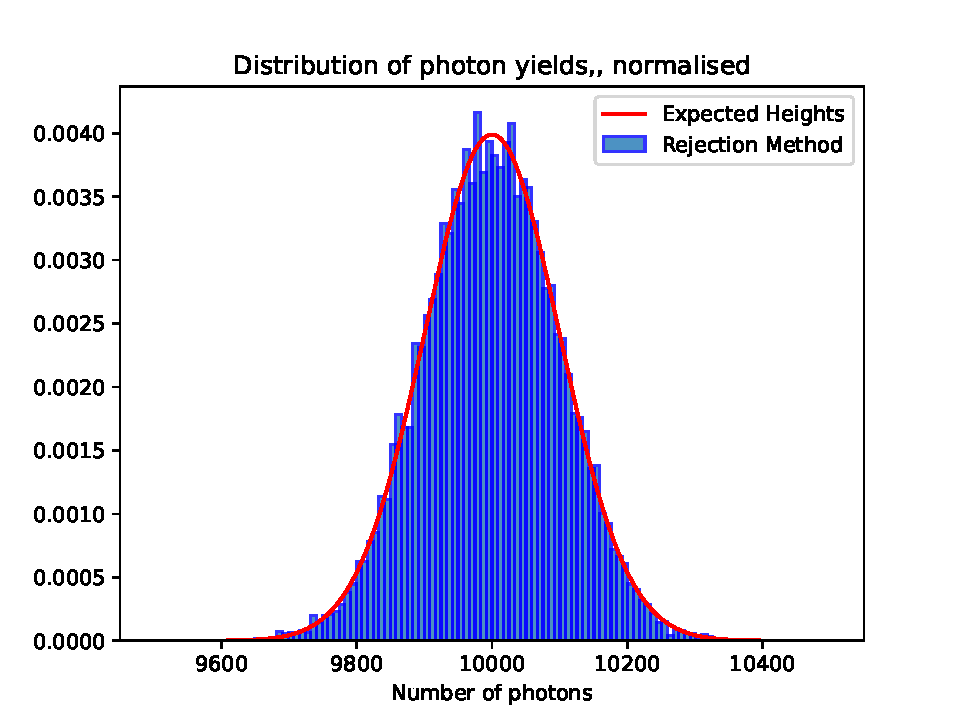
\includegraphics[width=.6\textwidth]{Plots/q1a.pdf}
                    \caption{Normalised distribution of photon yields. Expected heights are given by the Gaussian distribution in \cref{eqn:gaussian}.}
                    \label{fig:q1a}
                \end{center}
            \end{figure}
            
            \item The average yield was calculated to be \num[]{9999.4266}, which is round about what we expect.
            
            \item We found the variance to be \num{10020.466}. The assumed distribution has a variance of \num{10000}, so this is close, but it's hard to put an uncertainty on it so we can't say whether it's reasonable or not.
        \end{enumerate}

        \item We plot the distribution that photon momentum magnitudes obey, namely the Boltzmann distribution:
        \begin{equation}
            P(p)\propto p^2 e^{-p/T}
            \label{eqn:momentum magnitudes}
        \end{equation}

        \Cref{fig:q1b_unnormalised} shows the unnormalised distribution. Note that we plot it only on $p\in[0,30]$ as we can't plot it all the way to infinity, and it drops off appreciably by $p=30$. \\
        Integrating this distribution over $[0,\infty)$ we find a normalisation factor of 16, so we plot the normalised distribution in \cref{fig:q1b_normalised}, given by 
        \begin{equation}
            P(p)=\frac{p^2 e^{-p/T}}{16}.
            \label{eqn:boltzmann normalised}
        \end{equation}

        \begin{figure}[H]
            \begin{center}
                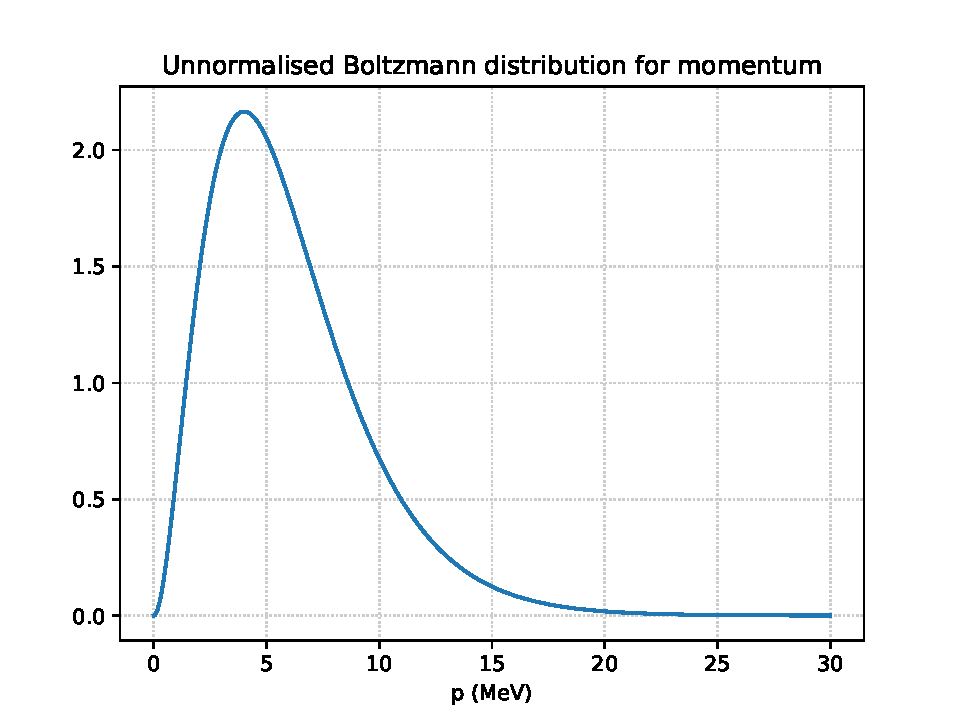
\includegraphics[width=.6\textwidth]{Plots/q1b_unnormalised.pdf}
                \caption{Unnormalised distribution of momentum magnitudes, following the Boltzmann distribution from \cref{eqn:momentum magnitudes} with $T=\SI{2}{\mega\electronvolt}$. }
                \label{fig:q1b_unnormalised}
            \end{center}
        \end{figure}

        
        \begin{figure}[H]
            \begin{center}
                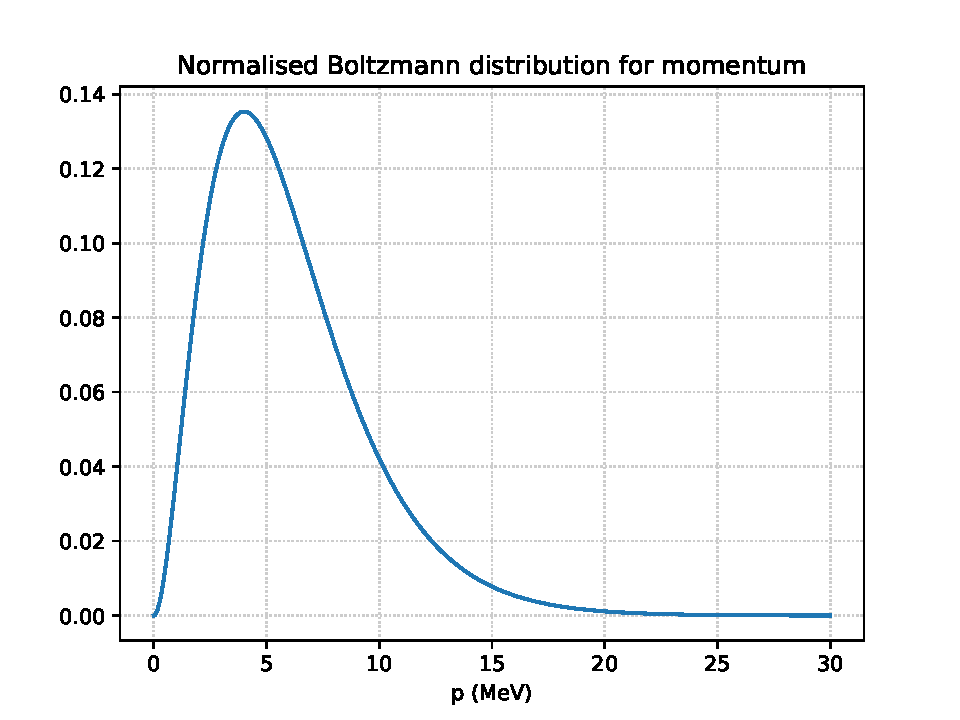
\includegraphics[width=.6\textwidth]{Plots/q1b_normalised.pdf}
                \caption{Normalised distribution of momentum magnitudes, once again following the distribution from \cref{eqn:momentum magnitudes} with $T=\SI{2}{\mega\electronvolt}$, now divided by 16.}
                \label{fig:q1b_normalised}
            \end{center}
        \end{figure}
        
        \item We now generate a set of random photon momentum magnitudes according to the distribution found above, specifically the normalised version. The number of photons to generate for is given by the first generated number in 1. a).
        
        \begin{enumerate}
            \item We plot the histogram in \cref{fig:q1c}
            \begin{figure}[h]
                \begin{center}
                    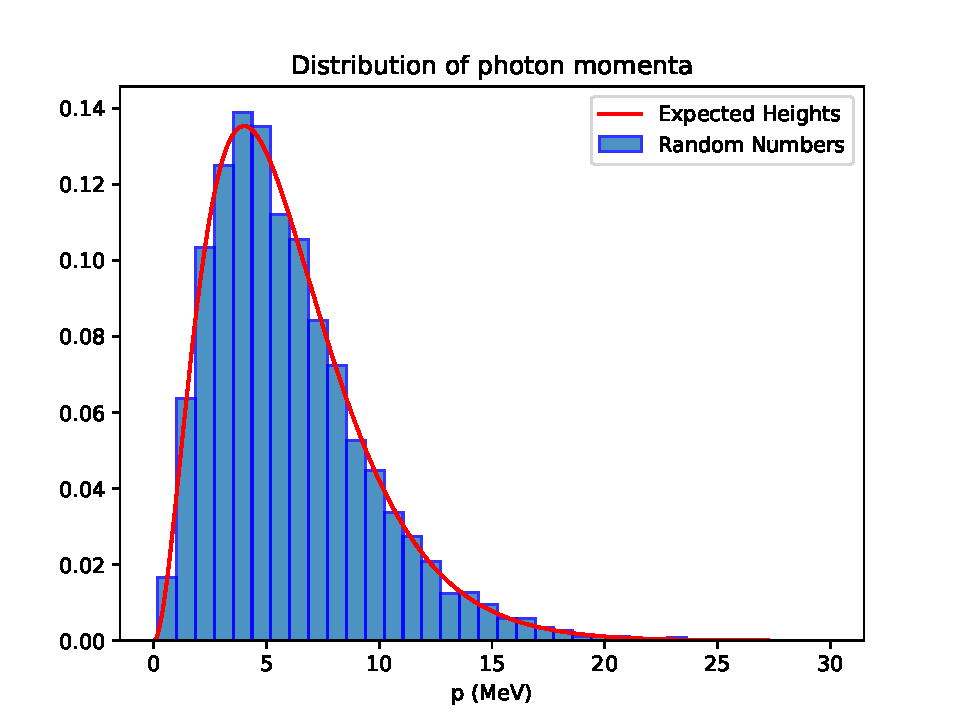
\includegraphics[width=.6\textwidth]{Plots/q1c.pdf}
                    \caption{Distribution of photon momentum magnitudes $p$, generated according to \cref{eqn:boltzmann normalised}, for \num{9759} photons. The expected heights are of course given by \cref{eqn:boltzmann normalised} as well.}
                    \label{fig:q1c}
                \end{center}
            \end{figure}

            \item The average $p$ was found to be \SI{5.9985}{\mega\electronvolt}.
            
        \end{enumerate}

        \item In order to derive the distributions governing emission angles $\theta$ and $\phi$, we must consider that isotropic means there is no preferred direction of emission, so any direction is equally likely. So, there is no $\theta$ or $\phi$ dependence on the probability for emission in some solid angle $d\Omega$, where we have the usual $d\Omega=\sin\theta d\theta d\phi$. We could write this as 
        \begin{equation*}
            \int P(\Omega)d\Omega = 1.
        \end{equation*}
        We know the integral of $d\Omega$ is simply the surface area on the unit sphere, $4\pi$, so since $P(\Omega)$ has no $\theta$ or $\phi$ dependence we must have that $P(\Omega)=\frac{1}{4\pi}$. So we can compare the solid angle probability integrand with one that considers the two probabilities to not be linked:
        \begin{align*}
            \frac{1}{4\pi}\sin\theta d\theta d\phi&=P(\theta)P(\phi)d\theta d\phi \\
            \implies P(\theta)P(\phi)&=\frac{1}{4\pi}\sin\theta.
        \end{align*}
        Here we're going to wave our hands and use the fact that the random points must be uniform when going around the equator, so the integral of $P(\phi)$ should be 1 and should not have any dependence. Thus we get 
        \begin{align*}
            P(\phi)&=\frac{1}{2\pi}\\
            P(\theta)&=\frac{1}{2}\sin\theta
        \end{align*}
        
        \item We aim to determine the expressions needed for the inverse method of generating random numbers. We begin with $\theta$.\\
        We can start with the general form of the inverse transform method
        \begin{equation}
            x_i=\int_{-\infty}^{y_i}P(y')dy'
            \label{eqn:general inverse method}
        \end{equation}
        where $x_i$ is a uniform number generated on $[0,1]$. We know that $\theta$ starts at 0, so we can write
        \begin{align*}
            x_i&=\int_0^{\theta_i}\frac 12 \sin\theta' d\theta'\\
            &=\frac 12 \left[-\cos\theta'\right]_0^{\theta_i}\\
            &=\frac 12 [-\cos\theta_i+1]\\
            \implies 2x_i-1&=-\cos\theta_i\\
            \implies \theta_i&=\arccos(1-2x_i).
        \end{align*}
        Now we can tackle $\phi$, once again starting \cref{eqn:general inverse method}. $\phi$ starts at $-\pi$, so we write
        \begin{align*}
            x_i&=\int_{-\pi}^{\phi_i}\frac{1}{2\pi}d\phi'\\
            &=\frac{1}{2\pi}[\phi']_{-\pi}^{\phi_i}\\
            &=\frac{1}{2\pi}[\phi_i+\pi]\\
            \implies2\pi x_i -\pi&=\phi_i\\
            \implies \phi_i &= 2\pi\left(x_i-\frac 12\right).
        \end{align*}

        \item We now use the inverse transform method to generate the distributions for $\theta$ and $\phi$ using the expressions found above. We will generate \num{9759} values as for the momentum magnitudes.
        \begin{enumerate}
            \item We plot the histograms
            
            \begin{figure}[h]
                \begin{center}
                    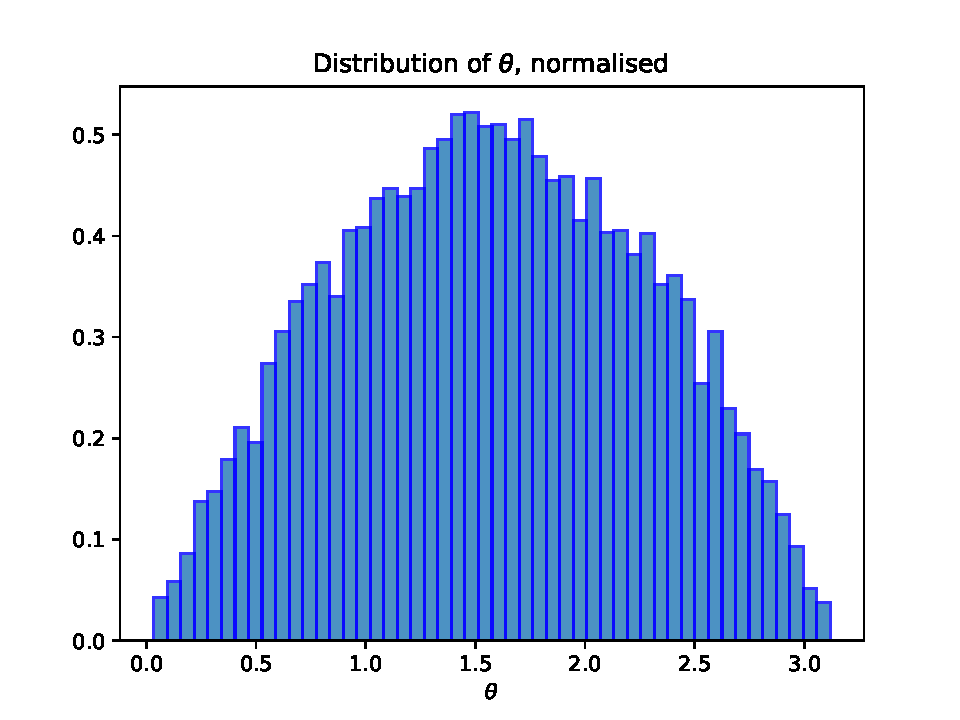
\includegraphics[width=.6\textwidth]{Plots/q1f_theta.pdf}
                    \caption{Distribution of \num{9759} random $\theta$ values generated with the inverse transform method.}
                    \label{fig:q1f theta}
                \end{center}
            \end{figure}

            \begin{figure}[h]
                \begin{center}
                    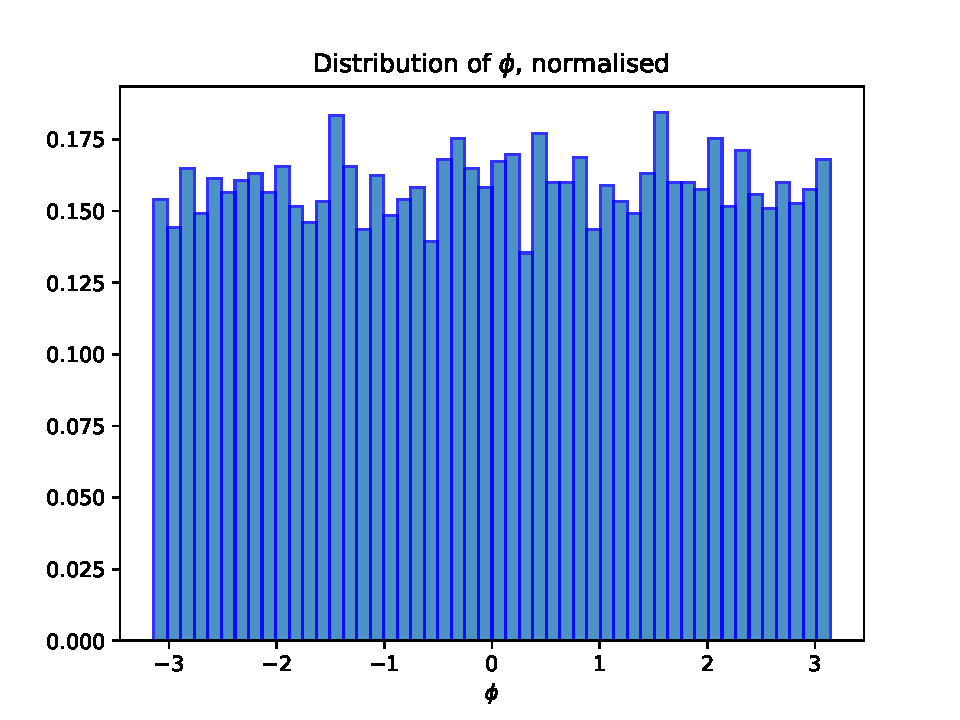
\includegraphics[width=.6\textwidth]{Plots/q1f_phi.pdf}
                    \caption{Distribution of \num{9759} random $\phi$ values generated with the inverse transform method.}
                    \label{fig:q1f phi}
                \end{center}
            \end{figure}
            
            \item We can find the average momentum in the $z$-direction for the first generated event. In spherical coordinates, the $z$ coordinate is given by 
            \begin{equation*}
                z=\cos\theta
            \end{equation*}
            so simply finding this value for each photon in the event and taking the mean we find $\langle p_z \rangle=\SI{-0.0007368}{\mega\electronvolt}$. 
            
        \end{enumerate}

        % -0.000736773019021856 z dir momentum
    \end{enumerate}

    \item We aim to solve the time-independent Schr\"odinger equation for an electron in a harmonic oscillator potential:
    \begin{equation}
        -\frac{\hbar^2}{2m}\frac{d^2\psi(x)}{dx^2}+\frac{1}{2}m\omega^2x^2\psi(x)=E\psi(x).
        \label{eqn:schrodinger harmonic}
    \end{equation}
    To do this, we will use the Numerov method. 
    \begin{enumerate}
        \item The Numerov method works to solve equations of the form
        \begin{equation}
            \frac{d^2y}{dx^2}+f(x)y=g(x).
            \label{eqn:numerov general}
        \end{equation}
        So, in order to use the Numerov method on \cref{eqn:schrodinger harmonic}, we must first identify $y=\psi(x)$, $g(x)=0$, and 
        \begin{equation}
            f(x)=\frac{2m}{\hbar^2}\left(E-\frac{1}{2}\frac{mc^2}{\hbar^2c^2}\hbar^2\omega^2x^2\right).
            \label{eqn:numerov f}
        \end{equation}
        Note here that we introduce a different looking potential term, but it is in fact the same, just easier to work with as we define $mc^2=\SI{5.11e5}{\electronvolt}$, $\hbar c=\SI{197.3}{\electronvolt\nano\metre}$, and $\hbar\omega=\SI{1}{\electronvolt}$. \\
        The Numerov method is a finite difference method, so we divide the region that we would like to work on into a grid of $x_i$ values with spacing $\Delta x$, and then use the notation $\psi_i=\psi(x_i)$ and $f_i=f(x_i)$. The derivation is long but eventually this leads us to the equations for finding a value for $\psi$ at a point as a function of values of $\psi$ at two other points:
        \begin{align}
            \psi_{i+1}&=\frac{\left(2-\frac{5}{6}\Delta x^2 f_i\right)\psi_i - \left(1+\frac{\Delta x^2}{12}f_{i-1}\right)\psi_{i-1}}{\left(1+\frac{\Delta x^2}{12}f_{i+1}\right)} \label{eqn:numerov update forwards}\\
            \psi_{i-1}&=\frac{\left(2-\frac{5}{6}\Delta x^2 f_i\right)\psi_i - \left(1+\frac{\Delta x^2}{12}f_{i+1}\right)\psi_{i+1}}{\left(1+\frac{\Delta x^2}{12}f_{i-1}\right)}. \label{eqn:numerov update backards}
        \end{align}
        These allow us to choose two starting values and then iterate across the grid, finding values of $\psi$, dependent on the value $E$ that sits in the $f_i$'s. Best practice when working with the Numerov method to solve the Schr\"odinger equation, since it has oscillatory solutions, is to work from the left and the right up to a classical turning point and match solutions at that point. In fact, this will help us decide whether a solution that we have found is in fact a solution to the Schr\"odinger equation. \\
        Stationary solutions to the Schr\"odinger equation, for well-behaved potentials, must be continuous both in their wavefunction and the first derivative of the wavefunction. For each energy value we try, we use Numerov to get a left and right solution, meeting at the turning point, and then match the value of the solutions by scaling the left solution. We then find the difference between the first derivatives at that point, using a central difference method, and define it as $d(E_0)$. For a valid solution, this $d(E_0)$ should be 0. Of course, this is a numerical scheme so we simply require it to be within some tolerance. We use $|d(E_0)|<\num{1e-4}$ as our condition. \\
        As a first approximation of the ground state energy, we found the energy of the ground state of a particle in an infinite well of width \SI{2}{\nano\metre}, as that seemed to be the length-scale of our problem. This came to be around \SI{0.1}{\electronvolt}, so we found $d(E_0)$ for a range of $E_0$ values starting from \SI{0.1}{\electronvolt} until the plot crossed zero 3 times. We could then find the ranges over which to search for the root by inspection. \Cref{fig:q2extra} shows the plot, and the ranges chosen were [0.1, 0.62], [1.3, 1.6], and [2.35, 2.6].

        \begin{figure}[h]
            \begin{center}
                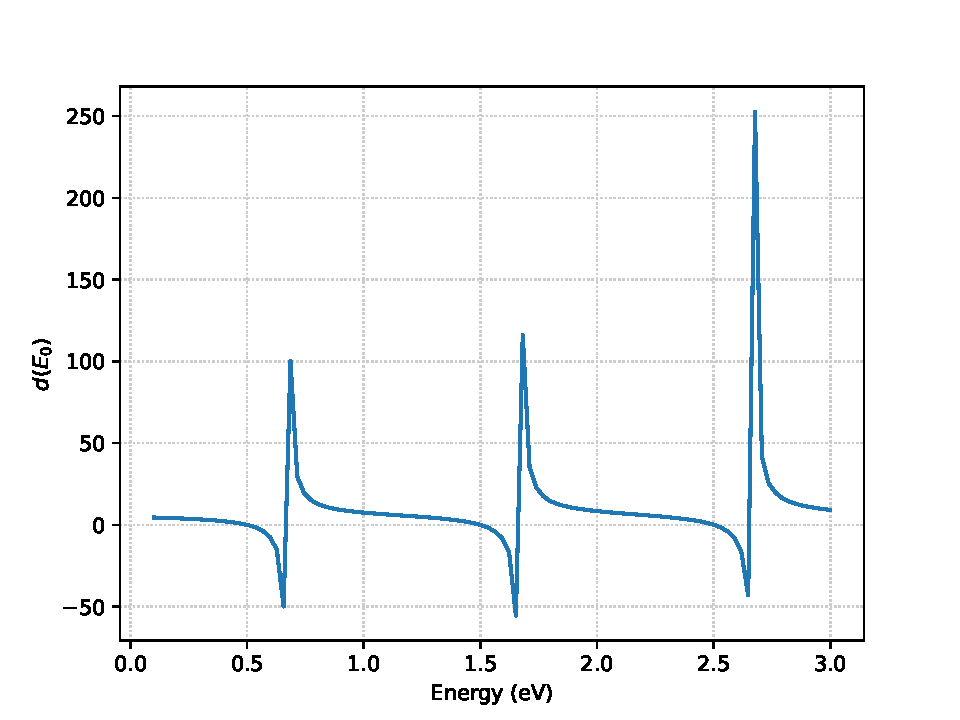
\includegraphics[width=.6\textwidth]{Plots/q2extra.pdf}
                \caption{Plot of $d(E_0)$ as a function of $E_0$, used to find the regions in which to search for zeros.}
                \label{fig:q2extra}
            \end{center}
        \end{figure}

        Using a simple Regula Falsi root-finding technique, we found the first three stationary state energies to be 
        \begin{equation*}
            E_0=\SI{0.50077}{\electronvolt},\quad E_1=\SI{1.5010}{\electronvolt},\;\;\mathrm{and}\;\; E_2=\SI{2.5029}{\electronvolt}.
        \end{equation*}
        
        \item Now, in order to find the stationary state wavefunctions corresponding to the energies found above, we simply input those energies into our Numerov method and combine the left and right solutions to get a solution on the whole space. Importantly the wavefunctions must be normalised in the usual sense, that the inner product of it with its complex conjugate must be 1.\\
        In our case, that means the integral of $\psi^2$ over the region $[-1,1]$ nm must be 1. To do this, we simply summed the values of the wavefunctions at each point on the grid, squared, and multiplied by the grid spacing $\Delta x$. The wavefunction could then be divided by the square root of this to normalise it. Note that more sophisticated methods of integration could be used, such as Simpson's method, but using them didn't show an appreciable difference, so the easier option was used.\\
        The wavefunctions are shown in \cref{fig:q2b} where each wavefunction is shifted up by its energy value in order to better show off its characteristics and relationship to the potential $V(x)$. 


        \begin{figure}[h]
            \begin{center}
                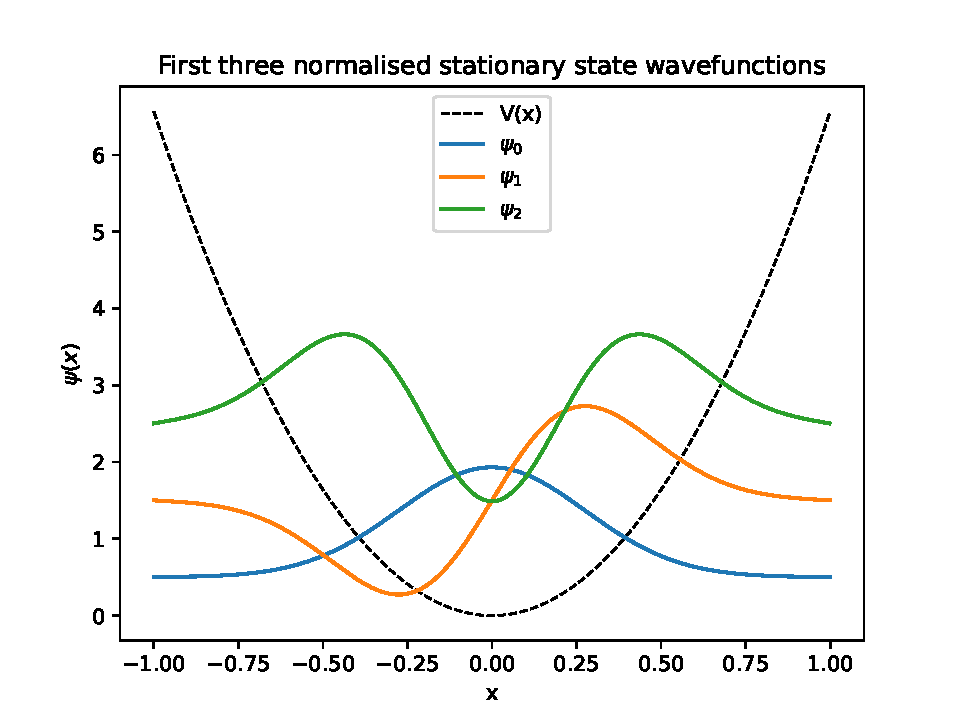
\includegraphics[width=.6\textwidth]{Plots/q2b.pdf}
                \caption{Plot of the first three stationary state wavefunctions, normalised, and shifted up by their energy for a better viewing experience. }
                \label{fig:q2b}
            \end{center}
        \end{figure}
        
        \item We can compare our energy values to the exact results, which we know to follow $E_n=\hbar\omega\left(n+\frac 12\right)$. We see up to 3 significant figures, our results agree with the exact values of $\frac 12$, $\frac 32$, and $\frac 52$. We have made no uncertainty analysis so it's hard to put a number to how good the values are, but trying with a smaller tolerance didn't seem to improve results beyond what we have, so there seems to be some systematic error. This is more than likely to be the $\mathcal{O}(\Delta x^6)$ truncation error in the Numerov method as we didn't use that many points in our grid, but we haven't explored that avenue.\\
        The form of the wavefunction is harder to analytically compare to the exact value, but upon inspection the numerical scheme has produces things of the right form, at least. The normalisation might not be entirely accurate as we normalised over [-1,1], not the entire $x$-axis, but it's hard to tell.
        
    \end{enumerate}

\end{enumerate}

\end{document}